\subsection{Time Projection Chamber}
%\writer{Paul Colas, Akira Sugiyama}{3}

The ILD TPC R\&D is being conducted mainly within the LCTPC Collaboration \cite{ild:bib:TPC_lctpc}. The history of these developments is described in the R\&D liaison report of the Linear Collider Collaboration~\cite{ild:bib:TPC_liaison} which contains many references (pp 36-60).

The workhorse for validation of detector prototypes and operational conditions is the TPC test set-up installed permanently in the DESY test beam~\cite{ild:bib:TPC_desytb} (Figure~\ref{fig:det:TPC_test_setup}). The TPC is situated in a superconducting magnet providing a magnetic field of 1 Tesla, and the beam line is equipped with precise incident and outgoing particle beam telescopes allowing to quantify the TPC reconstruction precision as function of the particle parameters. The beam test set up is currently being upgraded with the high precision LYCORIS silicon telescope~\cite{ild:bib:TPC_lycoris}, and a new TPC field cage with reduced field distortion is being assembled.

\begin{figure}[t!]
\centering
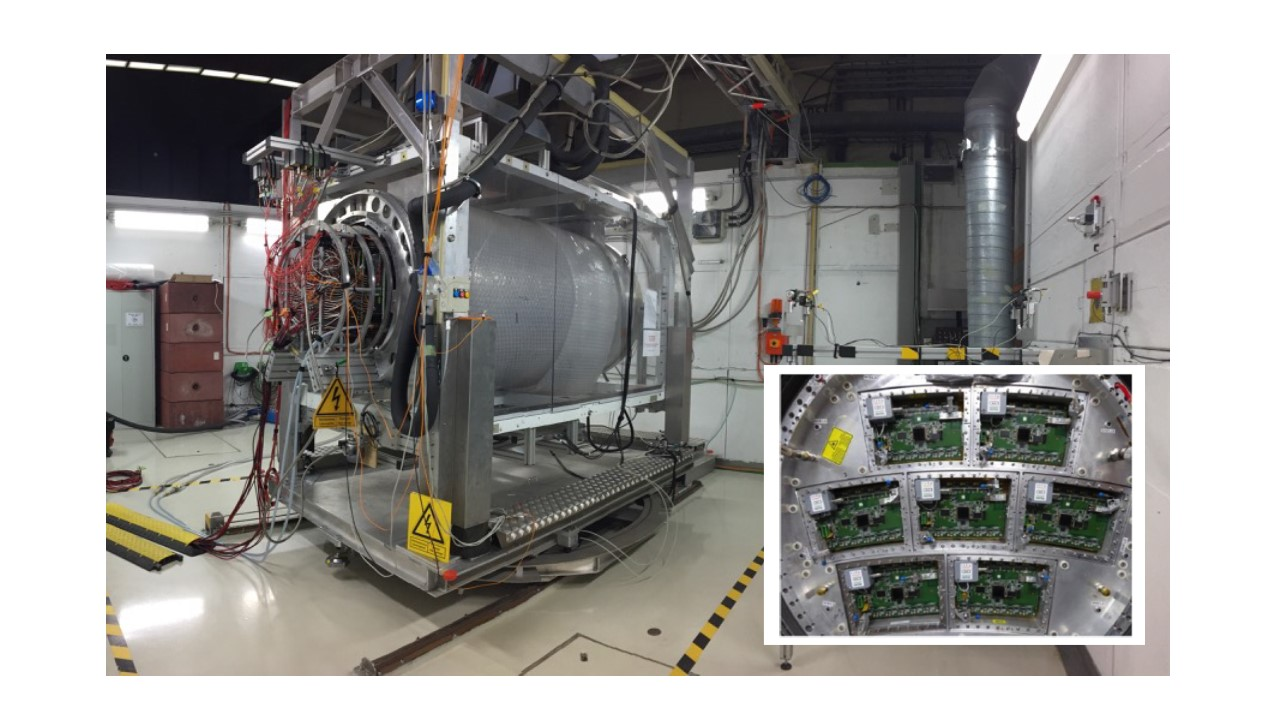
\includegraphics[width=1.0\hsize]{Detector/fig/TPC_test_setup.jpg}
\caption{The TPC test setup at DESY. The insert shows the geometrical structure of the TPC end cap which can host prototypes of detection planes.}
\label{fig:det:TPC_test_setup}
\end{figure}

Significant progress has been seen in the manufacturing process of detection modules for each of the readout options. A new Micromegas layout with resistive anodes has been shown to exhibit reduced boundary distortions~\cite{ild:bib:TPC_distortions}. The flatness of the GEM modules has been improved significantly, increasing the gain uniformity by a factor 2~\cite{ild:bib:TPC_GEMflatness}. Operational GridPix "QUAD" modules have been built based on the TimePix3 pixel chip~\cite{ild:bib:TPC_quad}. Recent prototypes of the three types of detection modules are shown in Figure~\ref{fig:det:TPC_prototypes}.  

\begin{figure}[t!]
\centering
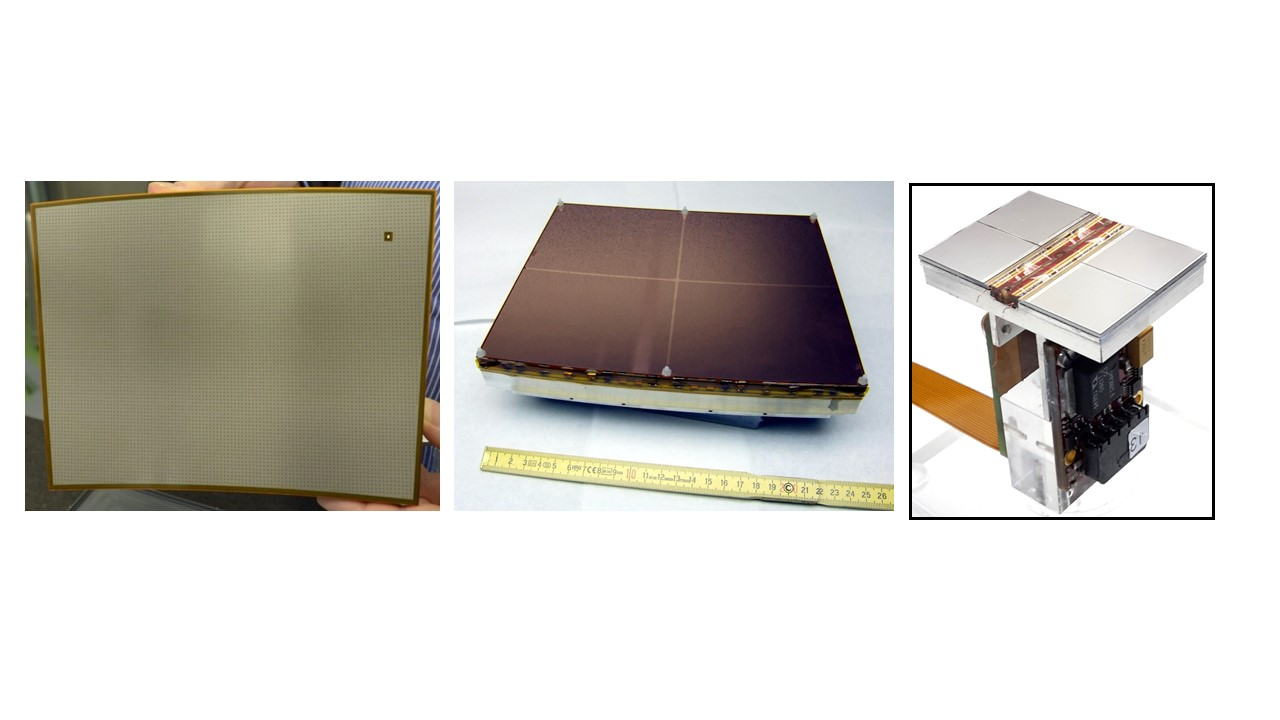
\includegraphics[width=1.0\hsize]{Detector/fig/TPC_prototypes.jpg}
\caption{TPC prototype detection modules for the three baseline technologies under consideration: Micromegas module (left), GEM module (middle) and GridPix QUAD module (right).}
\label{fig:det:TPC_prototypes}
\end{figure}

The performance of the three technologies has been measured in beam tests. Figure~\ref{fig:det:TPC_performances} shows the measured point resolution in 1~T magnetic field for drift distances from 0 to 0.6 m. This can be safely extrapolated to $\sim~100$ $\mu$m in a field of 3.5~T at a drift length of 2.3~m: the higher magnetic field reduces the transverse diffusion constant in the selected gas from 91~$\mu \mathrm{m} / \sqrt{\mathrm{cm}}$ to 30 $\mu \mathrm{m} / \sqrt{\mathrm{cm}}$, which compensates for the longer drift length compared to the prototype set-up. The dE/dx resolution determined by the truncated mean method has been measured to be $4.6\%, 4.5\%$ and $4.2\%$, respectively, for Micromegas, GEM and GridPix technologies. It improves to $3.8\%$ for GridPix using a cluster counting method. In conclusion the target requirement of a spatial resolution of $100 \mu$m in the transverse plane, and a dE/dx resolution better than 5\% have been reached in all options.   
\begin{figure}[t!]
\centering
\begin{subfigure}{0.48\textwidth}
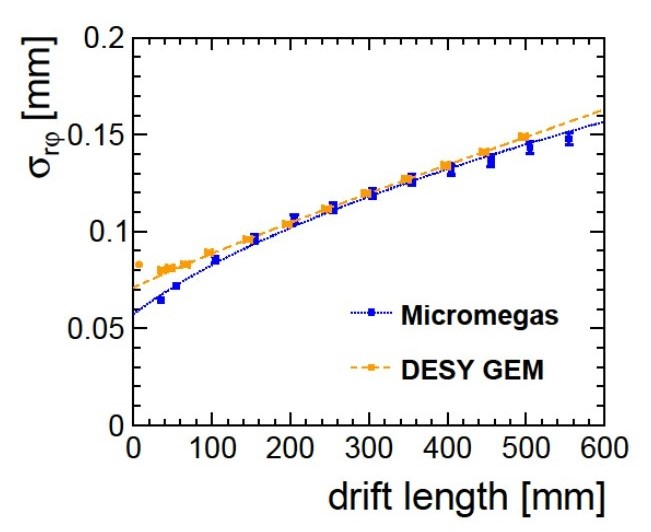
\includegraphics[width=1.0\hsize]{Detector/fig/TPC_performances_resolution.jpg}
\caption{}
\end{subfigure}
\begin{subfigure}{0.48\textwidth}
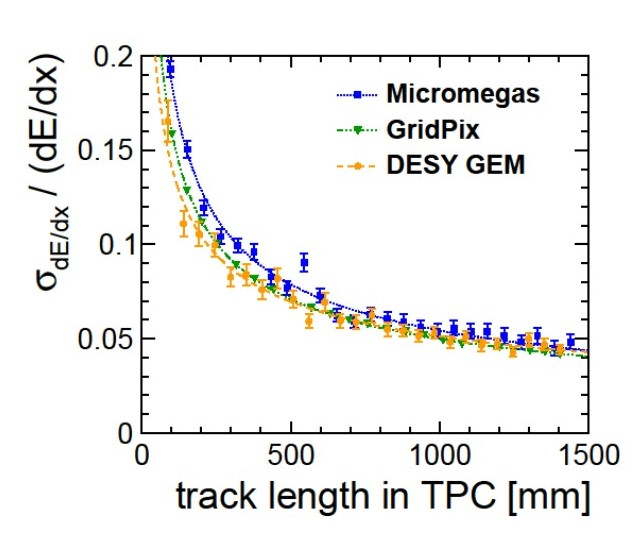
\includegraphics[width=1.0\hsize]{Detector/fig/TPC_performances_dedx.jpg}
\caption{}
\end{subfigure}
\caption{(a) Resolution on the track position in r$\phi$ as function of the drift length and (b) resolution on the ionisation loss dE/dx as function of the track length, for the three readout options under consideration.}
\label{fig:det:TPC_performances}
\end{figure}

Two-track separation has also been investigated. A $47\%~\rm{X_0}$ steel target was introduced near the TPC wall to produce multi-track events suitable for this study.
From these events a 2-hit separation distance of 4 to 6~mm was measured depending on the drift distance. An algorithm based on fitting the double-hit charge deposition with expected pad response function width allowed this separation distance to be reduced to 2~mm, with 1.3~mm pads (Figure~\ref{fig:det:TPC_separation}).

\begin{figure}[t!]
\centering
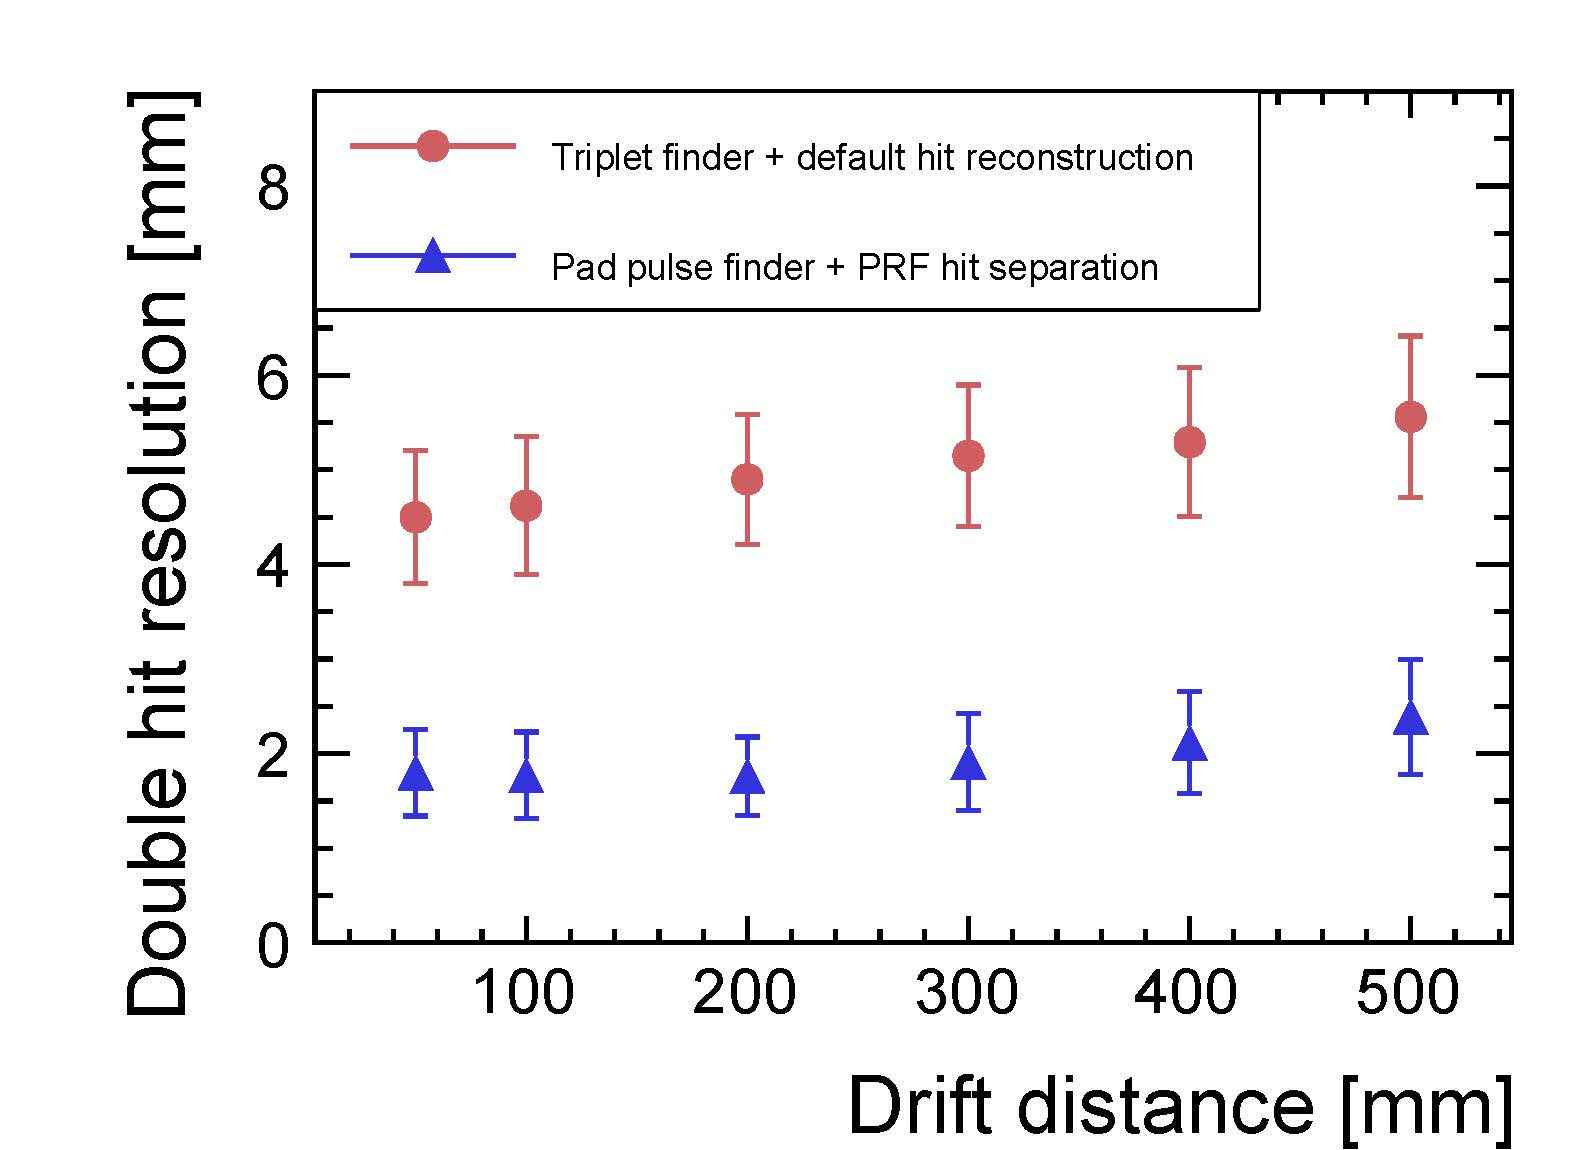
\includegraphics[width=0.55\hsize]{Detector/fig/TPC_separation.jpg}
\caption{2-hit separation as a function of the drift distance from beam test. Red dots are the results for standard hit reconstruction, blue triangles show the results of the improved algorithm. The data points shown correspond to the point where the separation efficiency has dropped to $50\%$, the bar describes the width of the error function, which is used to fit the transition region of the efficiency.}
\label{fig:det:TPC_separation}
\end{figure}

A challenging aspect of the TPC operation is the cooling of the readout end-caps, which must be realised with minimal dead material.  For this a double phase $\mathrm{CO}_2$ cooling system with thin low-material fluid pipes has been developed and is shown to perform adequately in test-beam experiments. 

Also critical for ultimate performance is the mitigation of the drift field distortions which may develop from the accumulation of ions migrating from the amplification region into the drift volume. For this an ion gating scheme based on a large aperture GEM foil (Figure~\ref{fig:det:TPC_gating} left) has been implemented and beam tested~\cite{ild:bib:TPC_gatinginbeam}. To prevent the positive ions created by the avalanches in the amplification device from flowing back to the drift space, a counter-field is created by applying a polarisation $\Delta V$ of -20 V between the faces of the gating GEM foil in between beam train crossings. During train crossings the voltage difference is reversed to +3 V, opening the way to the incoming electrons to be multiplied. 

Results from test bench measurements show that a good transparency for drift electron signals can be maintained while reducing the accumulation of ions in the drift volume by one order of magnitude~\cite{ild:bib:TPC_gatingpaper} (Figure~\ref{fig:det:TPC_gating} right).

\begin{figure}[t!]
\centering
\begin{subfigure}{0.40\textwidth}
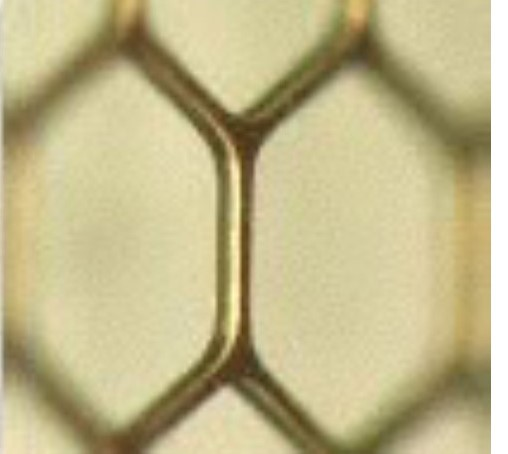
\includegraphics[width=1.0\hsize]{Detector/fig/TPC_gating_gem.jpg}
\caption{}
\end{subfigure}
\begin{subfigure}{0.48\textwidth}
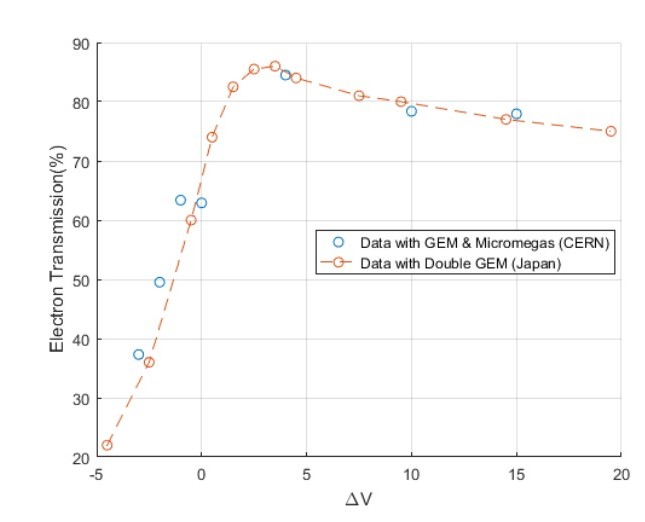
\includegraphics[width=1.0\hsize]{Detector/fig/TPC_gating_transparency.jpg}
\caption{}
\end{subfigure}
\caption{TPC gating: (a) detail of a GEM gating grid and (b) signal electron transparency with GEM gating as a function of the voltage difference (in Volts) across the two sides of the GEM plane in gate open mode.} 
\label{fig:det:TPC_gating}
\end{figure}

In conclusion all basic aspects of the TPC operation have shown to meet the requirements for an experiment at the ILC. 